\section{Arbeitsmarkt}
\begin{itemize}
	\item Arbeitslosigkeit existiert dann, wenn Haushalte bereit sind zum Marktlohn Arbeit anzubieten, diese aber nicht von den Unternehmen nachgefragt wird. (Dies kann in $"$regulierten$"$ Arbeitsmärkten der Fall sein.)
	\item Keine Arbeitslosigkeit herrscht dann, wenn Haushalte den Marktlohn als zu tief empfinden und deshalb keine Arbeit anbieten. (In einem $"$flexiblen$"$ Arbeitsmarkt kann es deshalb definitionsgemäss keine Arbeitslosigkeit geben.)
\end{itemize}

\begin{minipage}{12cm}
    Zwei Typen der Arbeitslosigkeit:
	\begin{itemize}
		\item \textbf{Sockelarbeitslosigkeit (X)}\newline
		 Anzahl der offenen Stellen ist gleich gross oder grösser als die Anzahl der Arbeitslosen (\textbf{strukturelle und friktionelle} Arbeitslosigkeit)
		\item \textbf{Konjukturelle Arbeitslosigkeit (Y)}\newline
		Anzahl der Arbeitslosen ist grösser als  die Anzahl der offenen Stellen
	\end{itemize}
\vspace{0.5cm}
Konjunkturelle Arbeitslosigkeit ensteht, wenn das BIP unterhalb der Kapazitätsgrenze liegt.
\end{minipage}
\begin{minipage}{5cm}
	\centering
	\includegraphics[width=4cm]{images/beveridge.jpg}
\end{minipage}
\flushleft

\subsection{Messung der Arbeitslosigkeit}
\begin{multicols}{2}
\includegraphics[width=\linewidth]{images/messung.png}
\columnbreak
\begin{description}
	\item[Bevölkerung:] Personen mit Aufenthaltsrecht
	\item[Erwerbsbevölkerung:] wollen arbeiten
	\item[Nichterwerbsbevölkerung:] wollen nicht arbeiten (StudentInnen, Hausmänner/-frauen, Wohlhabende, Auszeitnehmer)
	\item[Arbeitsproduktivität] Menge der produzierten Güter und Dienstleistungen pro Arbeitsstunde
	\item[Erwerbsquote:] inkl. Arbeitslos
	\item[Erwerbstätigenquote:] exkl. Arbeitslose
\end{description}
\end{multicols}

\subsection{Der flexible Arbeitsmarkt}
\begin{multicols}{2}
	\includegraphics[width=\linewidth]{images/felxibellohne.png}
	A: Angebot an Arbeit von Haushalten\\
	N: Unternehmen die Arbeiter suchen (auch Staat)
	\vfill\null
	\columnbreak
	\includegraphics[width=\linewidth]{images/flexibellohne2.png}
\end{multicols}

\subsection{Der regulierte Arbeitsmarkt}
	\includegraphics[width=0.8\linewidth]{images/fixelohne.png}

\subsection{Sockelarbeitslosigkeit}
\begin{multicols}{2}
\subsubsection{strukturelle Arbeitslosigkeit}
\label{sec:strukturelleArbeitslosigkeit}
Erklärungsfaktoren für strukturelle Arbeitslosigkeit
\begin{itemize}
	\item Mindestlöhne
	\item Zentralisierte Lohnverhandlungen
	\item Regulierungen bezüglich Anstellungen und Entlassungen
	\item Ausgestaltung der Arbeitslosenversicherung (Bezugshöhe)
	\item Regulierungen der Arbeitszeit
\end{itemize}
\vfill\null
\columnbreak
\subsubsection{friktionelle Arbeitslosigkeit}
\label{sec:friktionelleArbeitslosigkeit}
Erklärungsfaktoren für friktionelle Arbeitslosigkeit
\begin{itemize}
	\item Ausgestaltung der Arbeitslosenversicherung (Bezugsdauer)
	\item Zeitspanne bis Finden einer neuen Stelle
\end{itemize}
\end{multicols}

\subsection{Arbeitsmarktpolitik}
Zwei mögliche Ansätze zur Arbeitsmarktpolitik:
\begin{enumerate}
	\item Regulierung des Arbeitsmarktes:
	\subitem Diese Massnahmen beeinflussen die strukturelle Arbeitslosigkeit.
	\item Ausgestaltung der Arbeitslosenversicherung
	\subitem Diese Massnahmen beeinflussen die friktionelle und strukturelle Arbeitslosigkeit.
\end{enumerate}

\subsubsection{Arbeitsmarktpolitik der Schweiz}
Im Vergleich zu den Nachbarländern ist der Arbeitsmarkt in der Schweiz wenig reguliert:
\begin{enumerate}
	\item Mindestlöhne
	\subitem CH: keine branchenübergreifende Mindestlöhne
	\item Zentralisierte Lohnverhandlungen
	\subitem CH: nur dezentralisierte Vereinbarungen auf Branchenebene (ohne Staat)
	\item Regulierungen bezüglich Anstellungen und Entlassungen
	\subitem CH: wenig rechtliche Restriktionen
	\item Ausgestaltung der Arbeitslosenversicherung
	\subitem CH: setzt auf Wiedereingliederung
	\item Regulierung der Arbeitszeit
	\subitem CH: wenig rechtliche Restriktionen
\end{enumerate}

\subsubsection{Die ALV der Schweiz}
(obligatorisch ab 1977)\\
\begin{description}
	\item \textbf{Zwei Elemente}
	\begin{itemize}
		\item Passiver Teil: Zahlung eines Lohnersatzes
		\item Aktiver Teil: Arbeitsmarktrechtliche Massnahmen (Wiedereingliederung)
	\end{itemize}
	\item \textbf{Komponenten}
	\begin{itemize}
		\item Bezugsdauer: bis 90 Taggelder für Beitragsbefreite, bis 200 Taggelder für unter 25-jährige und bis 520 Taggelder für über 55-jährige
		\item maximal versicherbarer Lohn: 148200.-
		\item Höhe des Taggeldes: 70-80\% bis versicherbarer Lohn
		\item Beitragsdauer: 12 bis 24 Monate innerhalb der letzten 2 Jahre
	\end{itemize}
	\item \textbf{Finanzierung}
	\begin{itemize}
		\item 2.2\% der Lohnsumme bis 126000.-
		\item 1\% Solidaritätsbeitrag für die Lohnbestandteile ab 126000.-
	\end{itemize}
\end{description}

\begin{multicols}{2}
\subsubsection{Erhöhung der Sockelarbeitslosigkeit in der Schweiz}
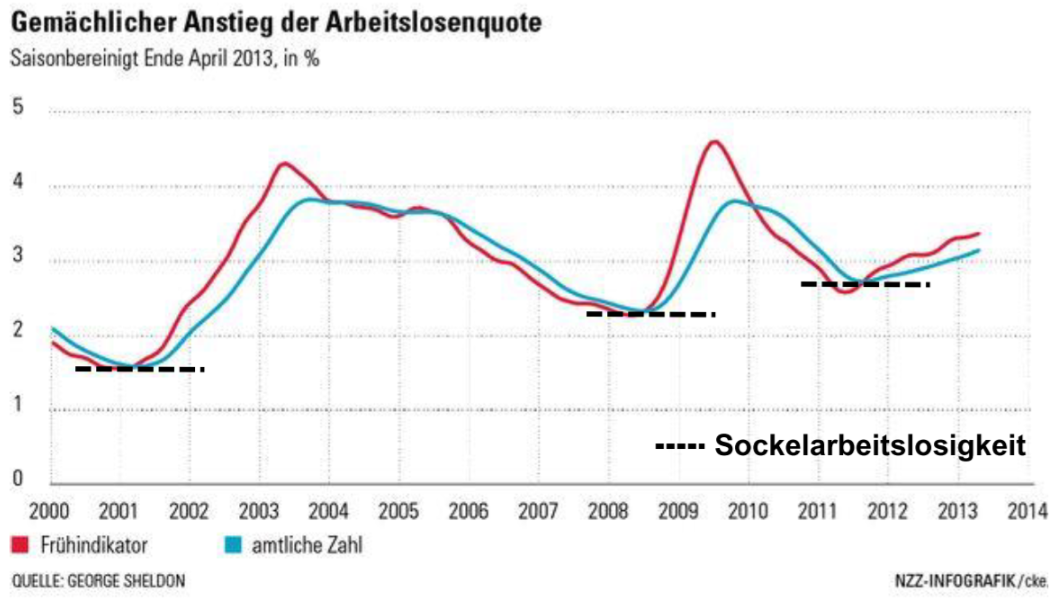
\includegraphics[width=\linewidth]{images/sockelarbeitslosigkeit.png}
\vfill\null
\columnbreak
\subsubsection{Regulierungsdichte ausgewählter Länder (2004)}
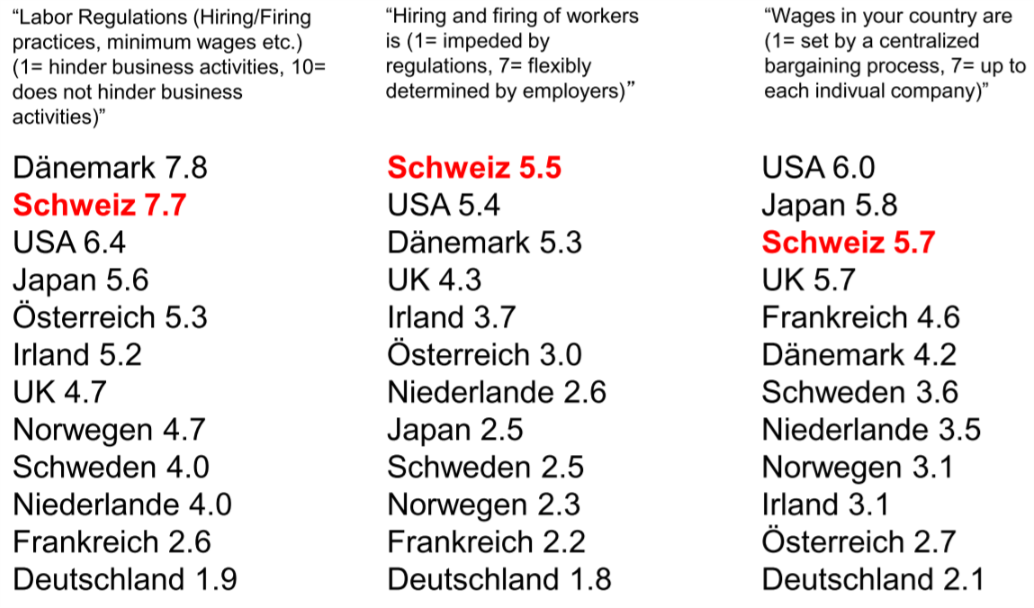
\includegraphics[width=\linewidth]{images/regulierungsdichte.png}
\textbf{Flexible Arbeitsmärkte erholen sich schneller!}
\end{multicols}

\subsubsection{Der Arbeitsmarkt in Frankreich}
Frankreichs Regierung hat im April 2015 eine Arbeitsmarktreform verabschiedet, die diese Bezeichnung aber kaum verdient. Unter anderem soll das System der Arbeitnehmervertretung vereinfacht werden.\\
Der französische Arbeitsmarkt leidet nicht nur unter einem scharfen Kündigungsschutz, überdurchschnittlich hohen Mindestlöhnen und Sozialabgaben, wie die OECD auch in ihrem neusten Länderbericht beanstandete. Hinzu kommt, dass Tarifverhandlungen und auch auch die Arbeitnehmervertretung sehr zentralistisch geregelt sind.

\subsubsection{Revitalisierung des deutschen Arbeitsmarktes}

\textbf{Ausgangslage}\\
Die Arbeitslosigkeit in Deutschland erhöhte sich zu Beginn des neuen Jahrtausends von 7\% (2000) auf 12\% (2005). Ein Grund dafür war der im internationalen Vergleich stark regulierte Arbeitsmarkt.\\
\vspace{\baselineskip}
\textbf{$"$Agenda 2010$"$}\\
Am 14. März 2003 kündigte Gerhard Schröder einen Massnahmenplan zur Revitalisierung des Arbeitsmarktes unter dem Begriff $"$Agenda 2010$"$ an. Dieser beinhaltete u.a. folgenden Massnahmen:
\begin{itemize}
	\item Zusammenlegen der Arbeitslosen- und Sozialhilfe (Hartz IV)
	\item Deregulierung der Temporär-Arbeit
	\item Anreize zur Arbeitsaufnahme
	\item Kürzung der Bezugsdauer der "normalen" Arbeitslosengelder
	\item Darüber hinaus: Abweichung von Flächentarifverträgen (IG Metall)
\end{itemize}
\vspace{\baselineskip}
\textbf{Ergebnis}\\
Deutschland entwickelte sich in wenigen Jahren vom "kranken Mann Europas" zum europäischen Musterknaben. Die Sockelarbeitslosigkeit sank deutlich. Der Vergleich der Kennzahlen von 2005 und 2013 zeigt:
\begin{itemize}
	\item Die Arbeitslosenquote sank von 12\% auf 7\%. Davon werden 1.5\%-3\% direkt auf die Umsetzung der $"$Agenda 2010$"$ zurückgeführt.
	\item Rückgang der Anzahl der Hartz IV-Empfänger von 2.9\% auf 2\%.
	\item Marginale Zunahme des Niedriglohnsektors von 2.3\% auf 2.4\% (Beschäftigte mit weniger als 2/3 des Medianlohns).
	\item Kaum Zunahme der $"$atypischen$"$ Beschäftigung wie Teilzeitarbeit (5 Mio.), befristete (2 Mio.) oder geringfügig Beschäftigte (2 Mio.). Neu kommen aber die Zeitarbeitnehmer (ca. 0.9 Mio.) dazu.
	\item Rückgang des Gini-Koeffizienten (entspricht einer Abnahme der sozialen Ungleichheit).
\end{itemize}
\vspace{\baselineskip}
\textbf{Betriebsbedingte Kündigung}\\
Von einer betrieblich bedingten Kündigung spricht man, wenn sachliche Gründe zu einer Unternehmerentscheidung führen, die ihrerseits den Wegfall eines Arbeitsplatzes des betroffenen Arbeitnehmers oder eine Mehrzahl von Arbeitsplätzen zur Folge hat. Hierbei sind grundsätzlich Gründe zu unterscheiden, die von aussen auf das Unternehmen einwirken (bspw. Umsatzeinbussen, Wegfall von Aufträgen) und Gründe, die von Unternehmen selbst herbeigeführt werden (Organisationsentscheidungen, Umstrukturierung, Betriebsschliessung). Die Unternehmerentscheidung selbst wird dabei von den Arbeitsgerichten nur auf $"$offensichtliche Willkür oder Unsachlichkeit$"$ geprüft.\\
Bei betrieblich bedingten Gründen ist die Sozialauswahl gemäss § 1 Abs.3 KSchG (Kündigungsgesetz) zu beachten. Von mehreren vergleichbaren Arbeitnehmern ist der Arbeitnehmer zu kündigen, der die besten Sozialdaten hat, das heisst der \textbf{am wenigsten von den Folgen der Kündigung getroffen wird}. Als Kriterien der Sozialauswahl dürfen seit der Neufassung des Kündigungsschutzgesetzes ab 1.1.2004 ausschliesslich die Dauer der Betriebszugehörigkeit, das Lebensalter, bestehende Unterhaltspflichten und möglicherweise vorliegende Schwerbehinderung herangezogen werden.\\
$\rightarrow$ dem "Besten" muss gekündigt werden\\
$\rightarrow$ Umgehen: Tochterfirmen mit weniger als 10 Mitarbeitenden

\clearpage
\pagebreak


